%% This is an example first chapter.  You should put chapter/appendix that you
%% write into a separate file, and add a line \include{yourfilename} to
%% main.tex, where `yourfilename.tex' is the name of the chapter/appendix file.
%% You can process specific files by typing their names in at the 
%% \files=
%% prompt when you run the file main.tex through LaTeX.
%\chapter{Use Case 1 - Both Drug and Target Side} \label{Use Case}
\chapter{Langkah-langkah Penggunaan}
Pada bagian ini akan dijelaskan secara rinci langkah-langkah penggunaan Ijah Webserver. Langkah-langkah ini mengacu pada Use-case 1 (Plant-Disease).

\section{Memberikan Masukan \emph{(inputs)}}

\begin{figure}[H]
	\centering
	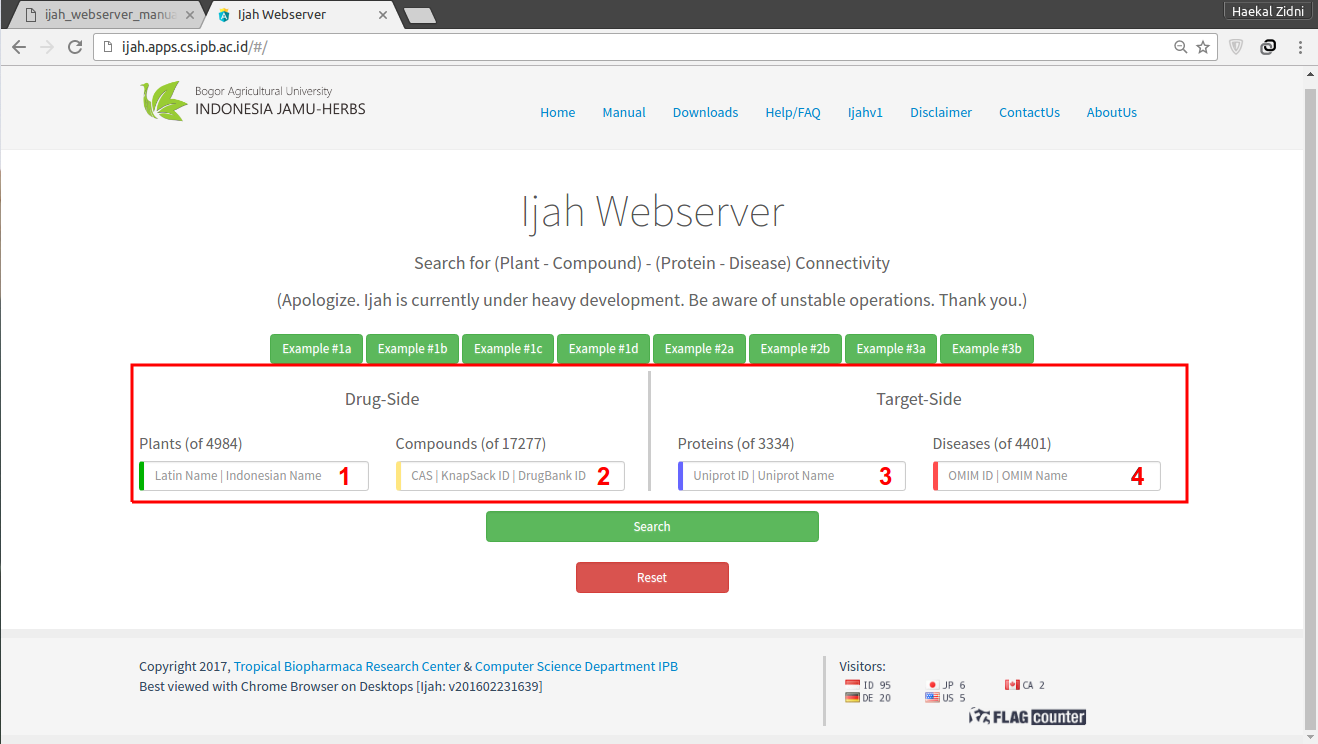
\includegraphics[scale=0.3]{ijah_input_form.png}
	\caption{Input Fields Ijah Webserver: Drug-Side - (1) Plants, (2) Compounds, Target-side - (3) Proteins, (4) Diseases}
	\label{fig:ijah_input_form}
	\end{figure}

	\subsection{Drug-side input}
	Pada saat memberikan masukan pada \emph(input fields) Ijah, perlu diperhatikan bahwa Ijah Webserver telah memiliki fitur \emph{autocomplete}, cukup mengetikkan sebagian dari nama latin atau nama Indonesia pada Plants atau salah satu ID dari input lainnya, maka saran yang mendekati hasil yang dimaksud sudah muncul. Untuk memulai, masukkan input pada Drug-side, misal tanaman.

	\begin{figure}[H]
		\centering
		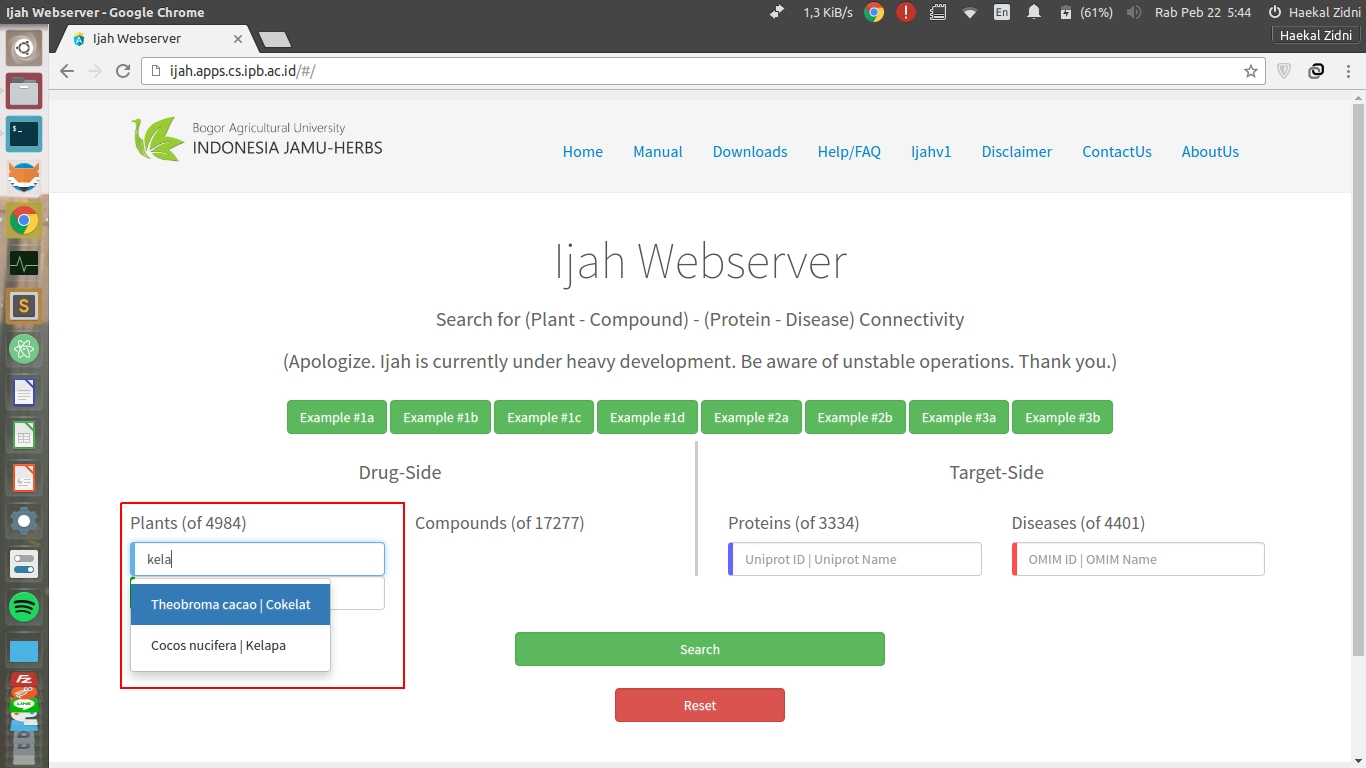
\includegraphics[scale=0.3]{ijah_autocomplete.png}
		\caption{Contoh saran dari \emph{autocomplete} ketika memasukkan `lida'}
		\label{fig:ijah_autocomplete_click}
		\end{figure}

	Untuk memilih, klik pilihan yang diinginkan. \textbf{Penting:} mengetikkan input secara manual hingga akhir tidak akan dianggap sebagai input yang \emph{valid}. Klik pilihan yang diinginkan agar masuk sebagai input yang\emph{valid}.

	Sebagai contoh, kita ingin memasukkan lidah buaya. Klik \mbox{\textbf{``Aloe Vera | Lidah Buaya''}} pada pilihan yang muncul. Jika sudah diklik, maka kotak akan terisi.

	\begin{figure}[H]
		\centering
		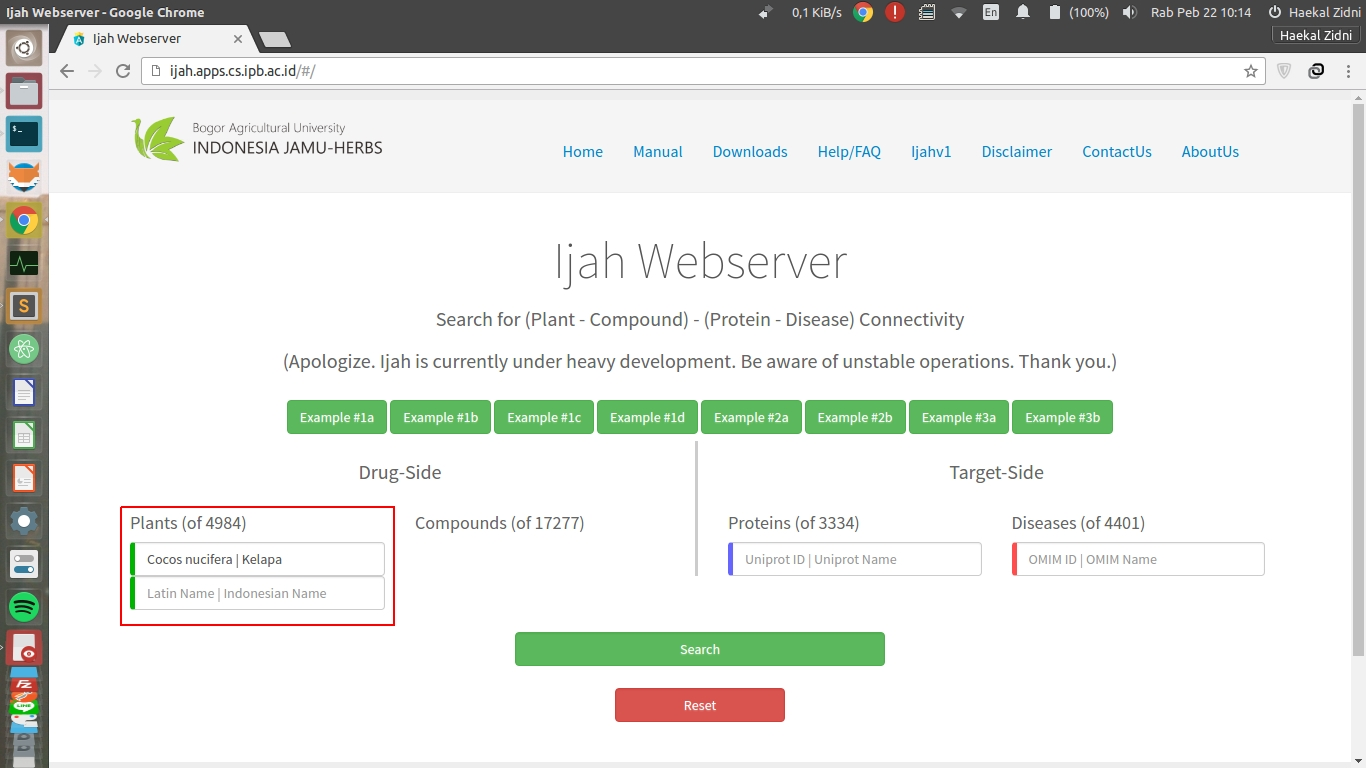
\includegraphics[scale=0.3]{ijah_autocomplete_complete.png}
		\caption{Setelah diklik input akan terlengkapi, dan kotak baru muncul di bawahnya}
		\label{fig:ijah_autocomplete_complete}
		\end{figure}

	Setelah memasukkan satu input, maka kotak baru akan muncul secara otomatis, jika kita ingin menambahkan input di kategori itu. Kotak baru akan terus muncul setelah satu input yang \emph{valid} masuk. Langkah ini berlaku untuk \emph{field} lain seperti Compounds, Proteins, dan Diseases.

	Perlu diperhatikan, pada gambar \ref{fig:ijah_autocomplete_complete}, saat input hanya berasal dari satu Side (dalam kasus ini hanya pada Drug-side), tombol eksekusi akan berlabelkan \textbf{Search} saja. Jika input terisi dari kedua Side maka label tombol akan berubah seperti pada gambar \ref{fig:ijah_autocomplete_complete2}.

	\subsection{Target-side input}
	Setelah memasukkan input dari Drug-side (dalam use-case ini memasukkan tanaman), maka dilanjutkan dengan memasukkan input dari Target-side. Cara memberikan masukan tetap sama. Kali ini sebagai contoh akan diinputkan disease \mbox{\textbf{``614292 | Myopia, high, with cataract and vitreoretinaldegeneration''}}

	\begin{figure}[H]
		\centering
		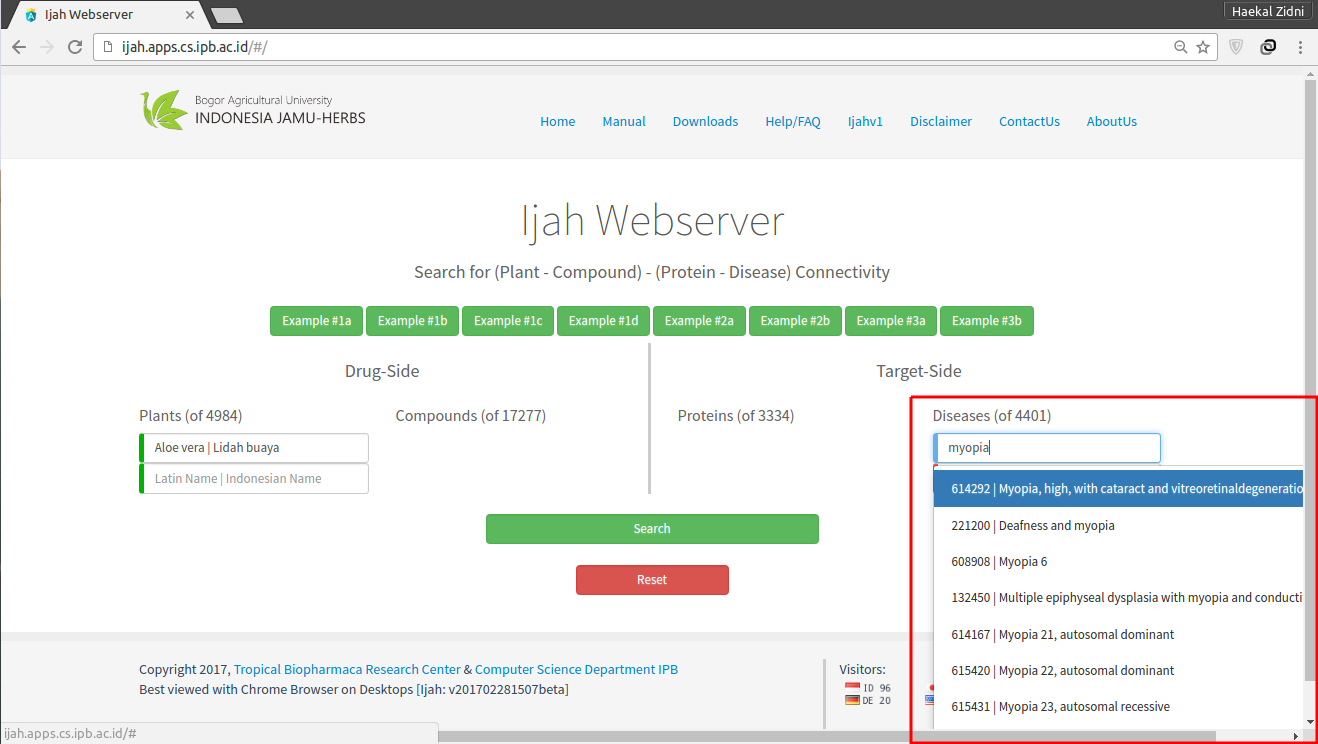
\includegraphics[scale=0.3]{ijah_autocomplete2.png}
		\caption{\emph{autocomplete} pada saat memasukkan Target berupa Disease}
		\label{fig:ijah_autocomplete_click2}
		\end{figure}

	\begin{figure}[H]
		\centering
		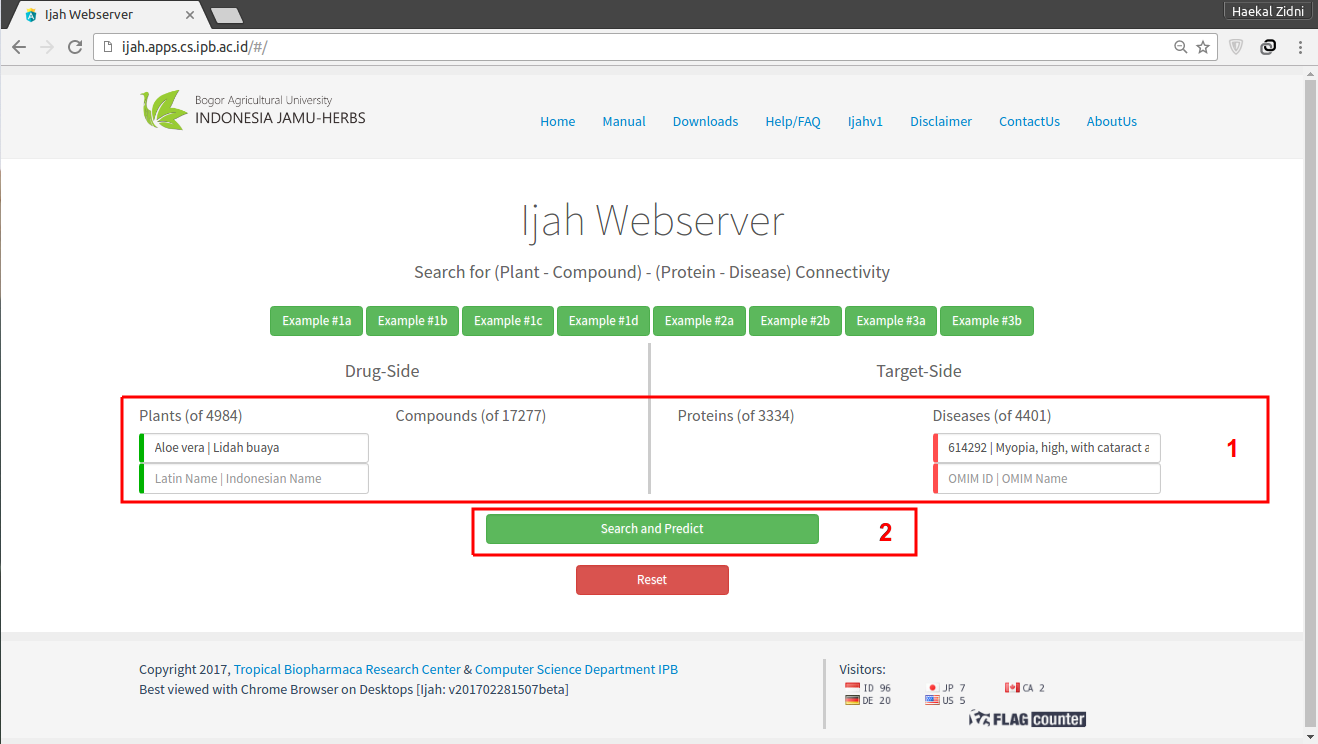
\includegraphics[scale=0.3]{ijah_autocomplete_complete2.png}
		\caption{(1) Input dari kedua sisi sudah lengkap. (2) Perhatikan tombol eksekusi yang berlabel \emph{textbf{Search and Predict}}}
		\label{fig:ijah_autocomplete_complete2}
		\end{figure}


\section{Memproses} \label{process}
Setelah memasukkan input, langkah berikutnya yaitu input dapat diproses. Setelah tombol eksekusi diklik, maka proses Search and Predict akan berjalan. Selama proses berjalan, akan muncul animasi seperti pada gambar \ref{fig:ijah_process_bounce}

\begin{figure}[H]
	\centering
	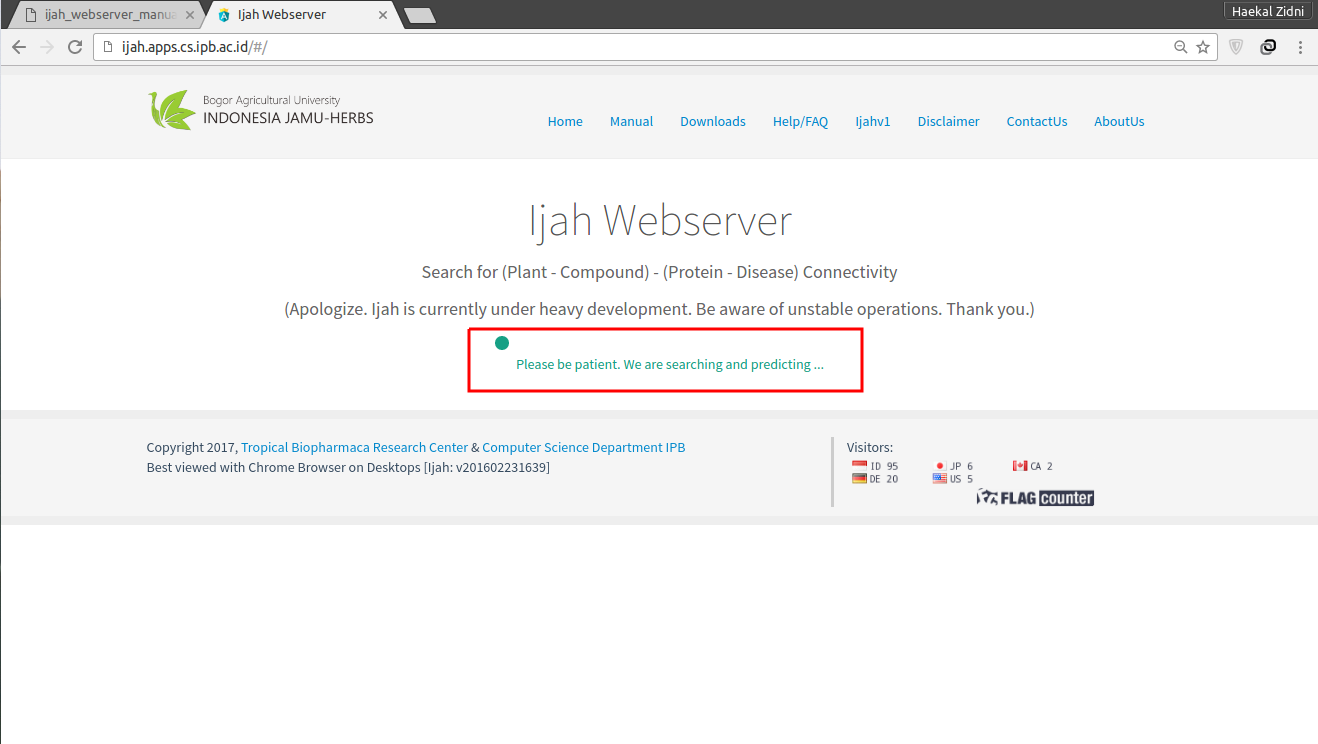
\includegraphics[scale=0.3]{ijah_process_bounce.png}
	\caption{Animasi saat proses Search and Predict sedang berlangsung}
	\label{fig:ijah_process_bounce}
	\end{figure}

\section{Membaca luaran \emph{(outputs)}}
Setelah proses selesai, maka luaran \emph{(output)} yang dihasilkan sudah dapat dibaca. Terdapat empat kategori \emph{output} yang dihasilkan, yaitu:
	
	\subsection{Summary} \label{summary}
	\begin{figure}[H]
	\centering
	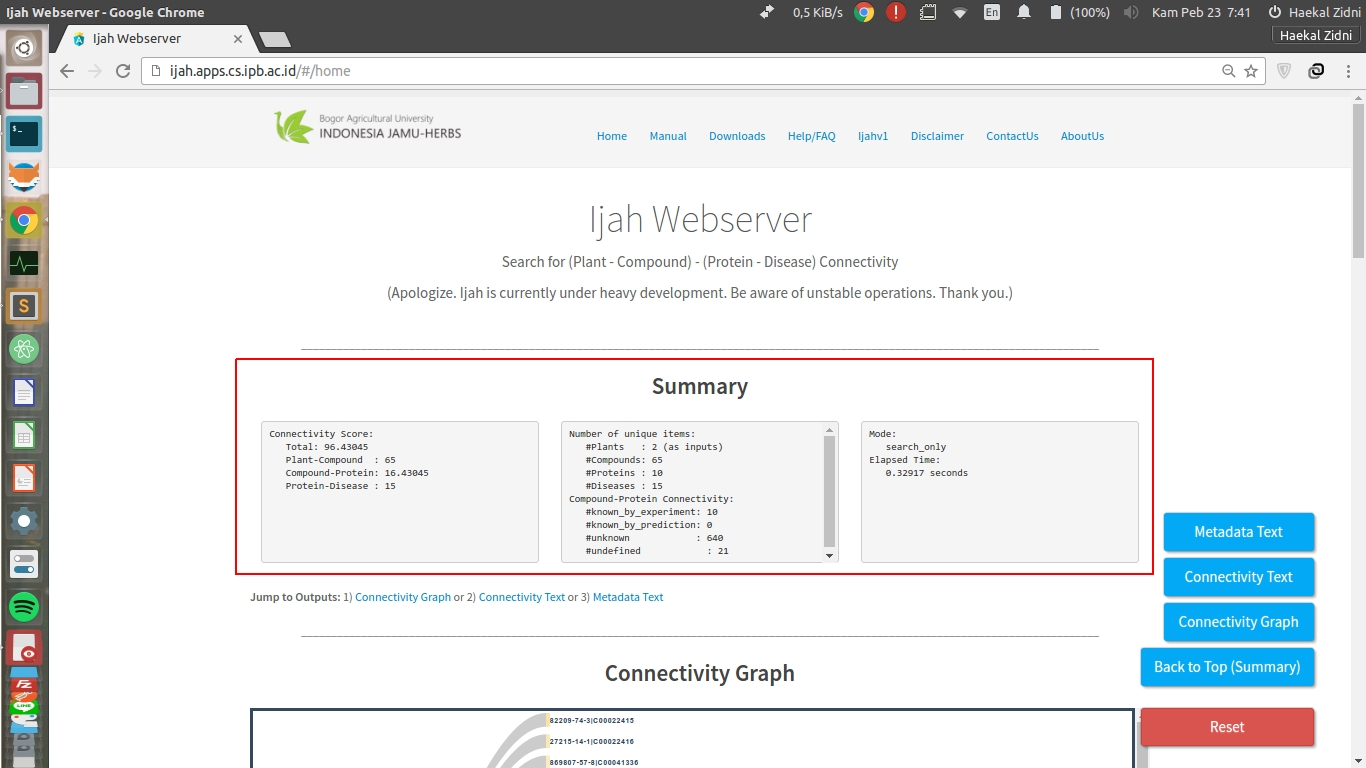
\includegraphics[scale=0.3]{ijah_output_summary.png}
	\caption{Output Summary}
	\label{fig:ijah_output_summary}
	\end{figure}
	
	Output Summary adalah ringkasan dari proses output, yang meliputi:
	\begin{itemize}
	\item \textbf{Minimum Connectivity Weight to Process} -- nilai minimum skor yang diproses, dapat diubah melalui filter yang akan dijelaskan di bagian \hyperref[nav]{Filter pada Navigasi}.
	\item \textbf{Connectivity Score} -- jumlah total dari nilai seluruh konektivitas (1 artinya 100\% terhubung, 0 tidak terhubung, di antara 1 dan 0 berarti hasil prediksi yang nilainya belum 100\%, seluruh keterhubungan dijumlah untuk mendapat nilai total).
	\item \textbf{Number of Unique Items} -- jumlah entitas unik (tidak termasuk pengulangan) yang terlibat dalam proses.
	\item \textbf{Compound-Protein Connectivity} -- jumlah konektivitas senyawa dan protein. \textbf{Known by experiment} artinya data sudah valid 100\%, berasal dari pangkalan data, sedangkan \textbf{Known by prediction} berarti konektivitas hasil prediksi algoritme, \textbf{Unknown} artinya konektivitas yang tidak diketahui baik dari pangkalan data maupun hasil prediksi algoritme.
	\item \textbf{Mode} -- mode proses, apakah Search saja atau Search and Predict.
	\item \textbf{Elapsed Time} -- waktu yang dihabiskan untuk menyelesaikan proses.
	\end{itemize}
	
	\subsection{Connectivity Graph} \label{graph}
	Connectivity Graph merupakan model output yang berupa \emph{multi-partite graph}, yaitu graf yang verteksnya terbagi menjadi beberapa partisi.

	\begin{figure}[H]
	\centering
	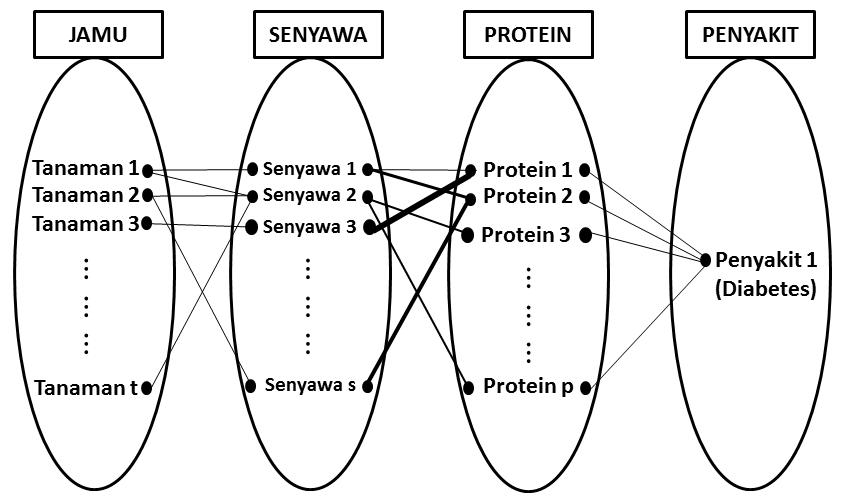
\includegraphics[scale=0.5]{multipartite-graph.png}
	\caption{Contoh \emph{multipartite graph}}
	\label{fig:multipartite-graph}
	\end{figure}

	\begin{figure}[H]
	\centering
	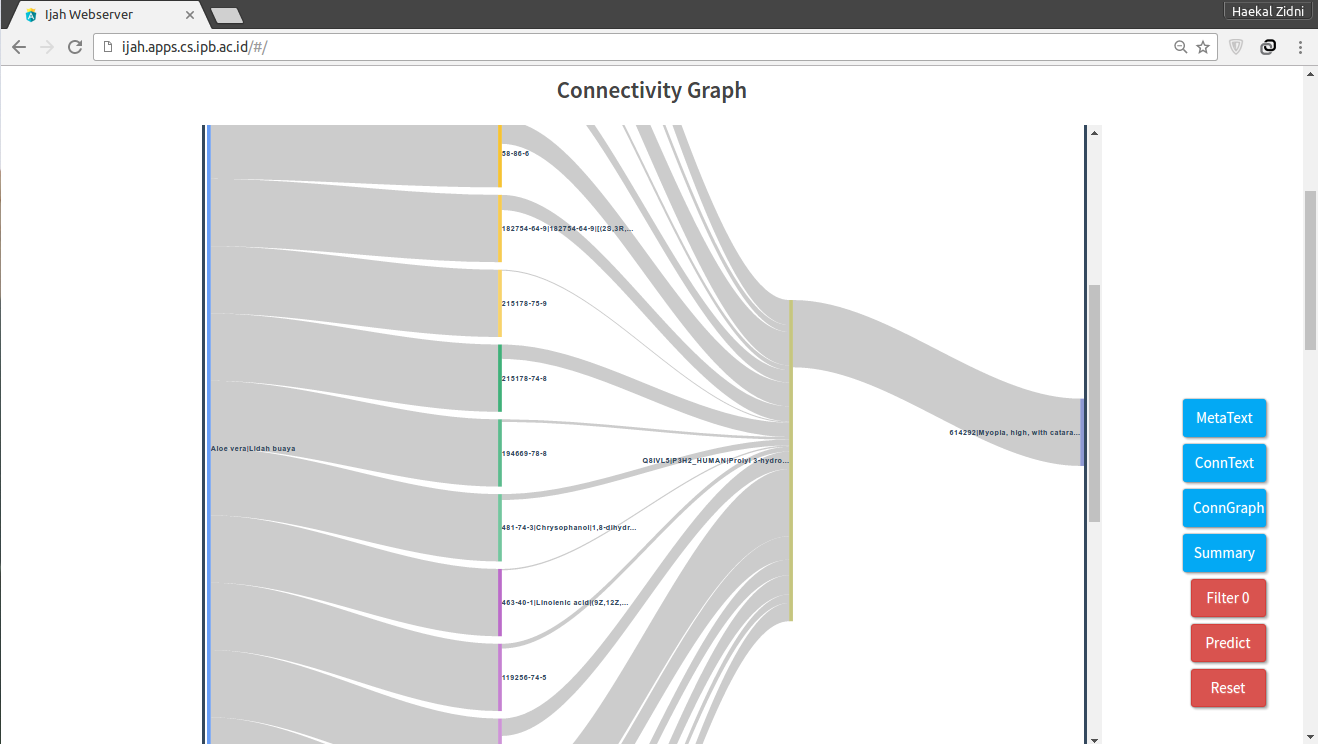
\includegraphics[scale=0.3]{ijah_output_graph.png}
	\caption{Connectivity Graph pada Ijah Webserver}
	\label{fig:ijah_output_graph}
	\end{figure}
	
	Pada model Connectivity Graph Output, terdapat vertex dari Plant ke Compound, Compound ke Protein, dan Protein ke Disease, ada 4 partisi pada graf ini.

	\begin{figure}[H]
	\centering
	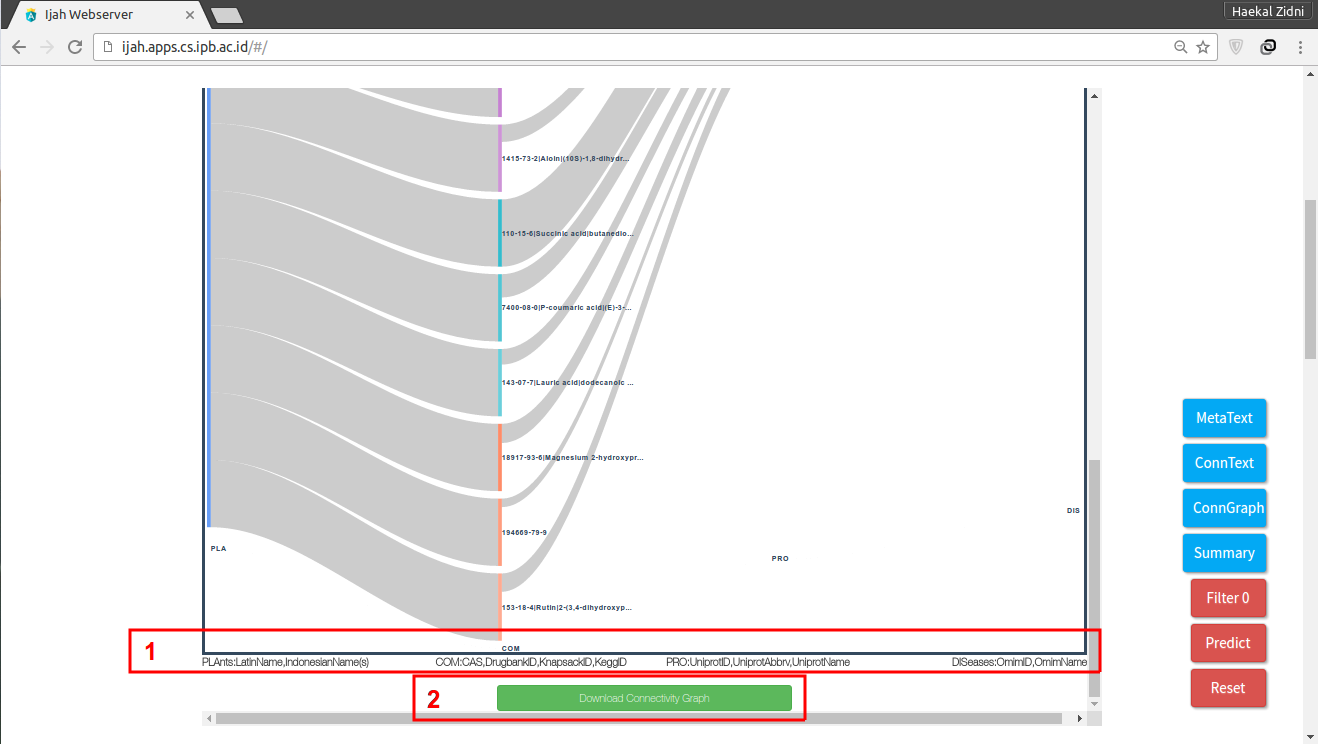
\includegraphics[scale=0.3]{ijah_output_graph_bottom.png}
	\caption{Bagian bawah Connectivity Graph -- (1) Keterangan Graf, (2) Tombol Download}
	\label{fig:ijah_output_graph_bottom}
	\end{figure}

	Pada bagian bawah dan atas graf terdapat panduan setiap partisi graf, dari paling kiri Plants (nama latin | nama Indonesia), lalu Compounds (dan IDnya (CAS, Drugbank, Knapsack, Kegg)), Proteins dan IDnya (nama Uniprot, singkatan (abbrv) Uniprot, ID Uniprot), dan Diseases beserta IDnya di paling kanan (ID dan nama OMIM).

	Navigasi graf dapat dilakukan dengan menggulir \emph{scrolling} ke atas dan bawah. Graf ini bisa didownload menggunakan tombol Download di bawah graf, dengan format gambar PNG.
	
	\subsection{Connectivity Text} \label{text}

	Selain dalam bentuk \emph{multipartite graph}, output juga dihasilkan dalam bentuk Connectivity Text, yaitu teks yang berisi konektivitas antar entitas

	\begin{figure}[H]
	\centering
	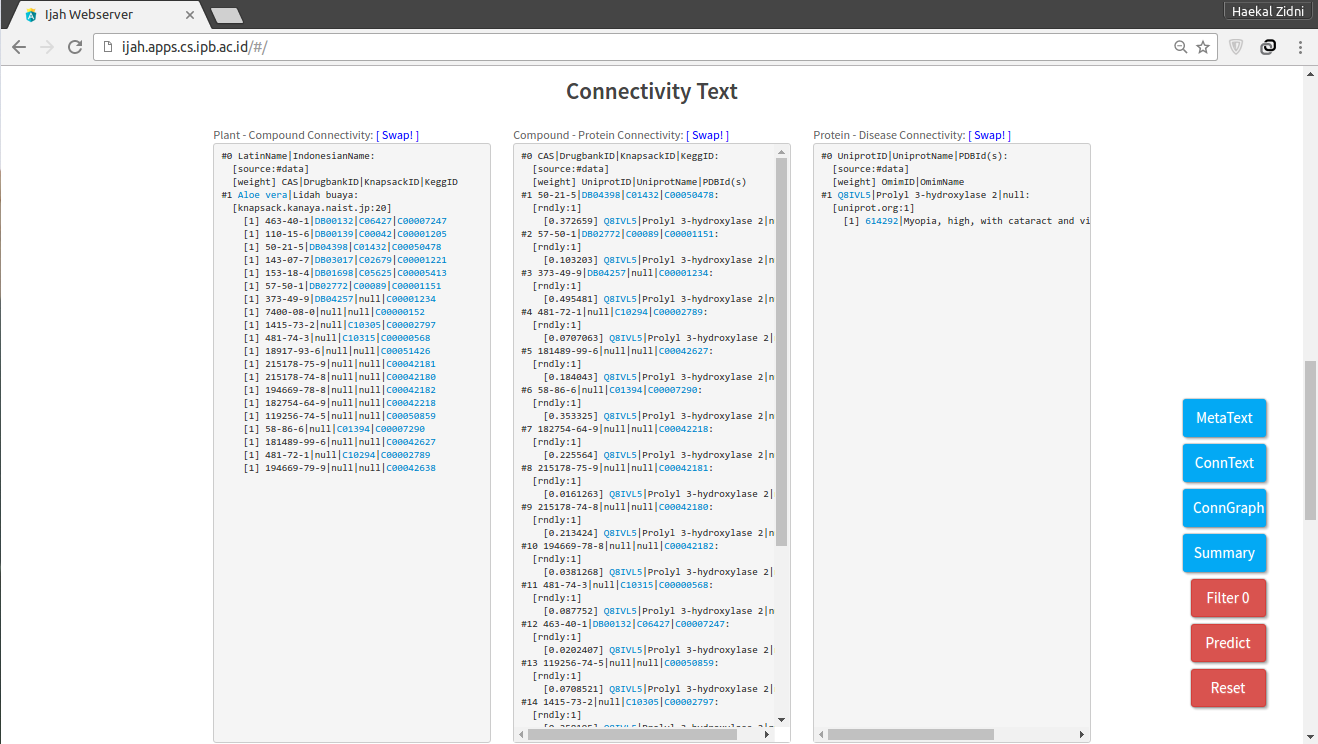
\includegraphics[scale=0.3]{ijah_output_text.png}
	\caption{Connectivity Text pada Ijah Webserver}
	\label{fig:ijah_output_text}
	\end{figure}	
	
	Isi pada output Text yaitu data konektivitas (nama dan ID entitas pertama), sumber data konektivitas, serta bobot nilai konektivitas (1 jika terhubung 100\% by experiment, jika by prediction nilainya akan bervariasi antara 0 sampai 1, lebih mendekati 1 maka lebih baik), lalu nama dan ID entitas keduanya.

	Pada output Text, dapat dilakukan \emph{swapping} konektivitas, misal dari Plant-Compound menjadi Compound-Plant. Hal ini dapat dilakukan dengan mengklik tombol \textbf{Swap!} di bagian atas tiap kotak konektivitas.

	\begin{figure}[H]
	\centering
	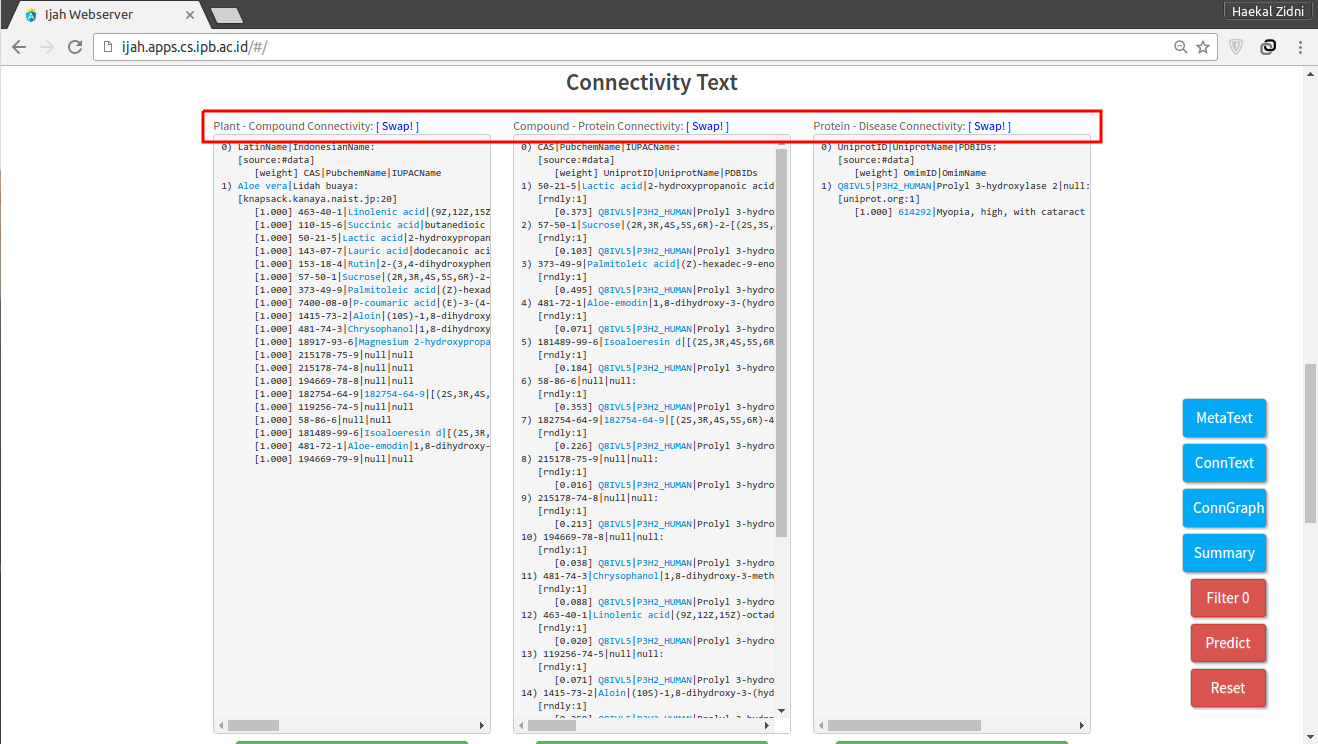
\includegraphics[scale=0.3]{ijah_output_text_swapbutton.png}
	\caption{Posisi tombol Swap untuk Connectivity Text}
	\label{fig:ijah_output_text_swapbutton}
	\end{figure}

	\begin{figure}[H]
	\centering
	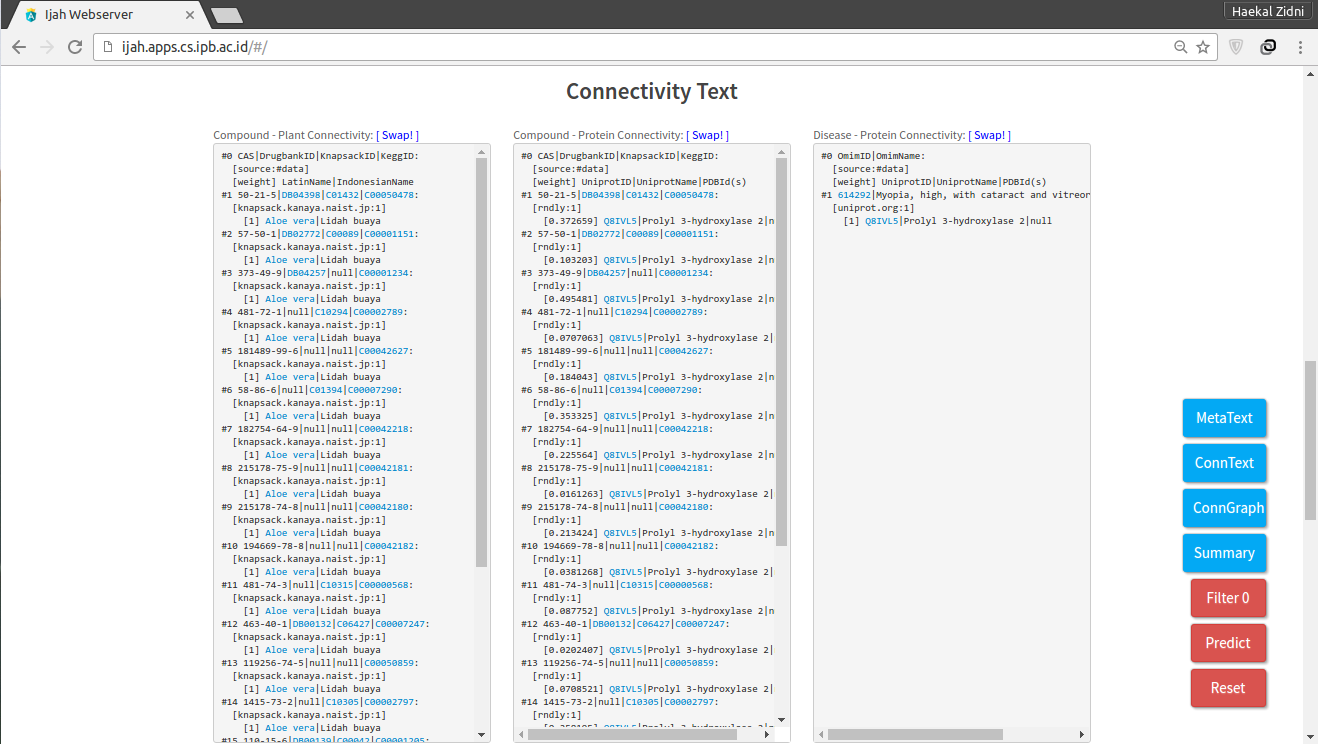
\includegraphics[scale=0.3]{ijah_output_text_swapped.png}
	\caption{Hasil Swapping pada Plant-Compound dan Protein-Disease. Perhatikan bahwa konektivitasnya berubah menjadi Compound-Plant dan Disease-Protein}
	\label{fig:ijah_output_text_swapped}
	\end{figure}

	Seperti Connectivity Graph, Connectivity Text juga memiliki tombol Download untuk mendownload file teks konektivitas ini. Download dilakukan per konektivitas sehingga terbagi menjadi tiga file.

	\begin{figure}[H]
	\centering
	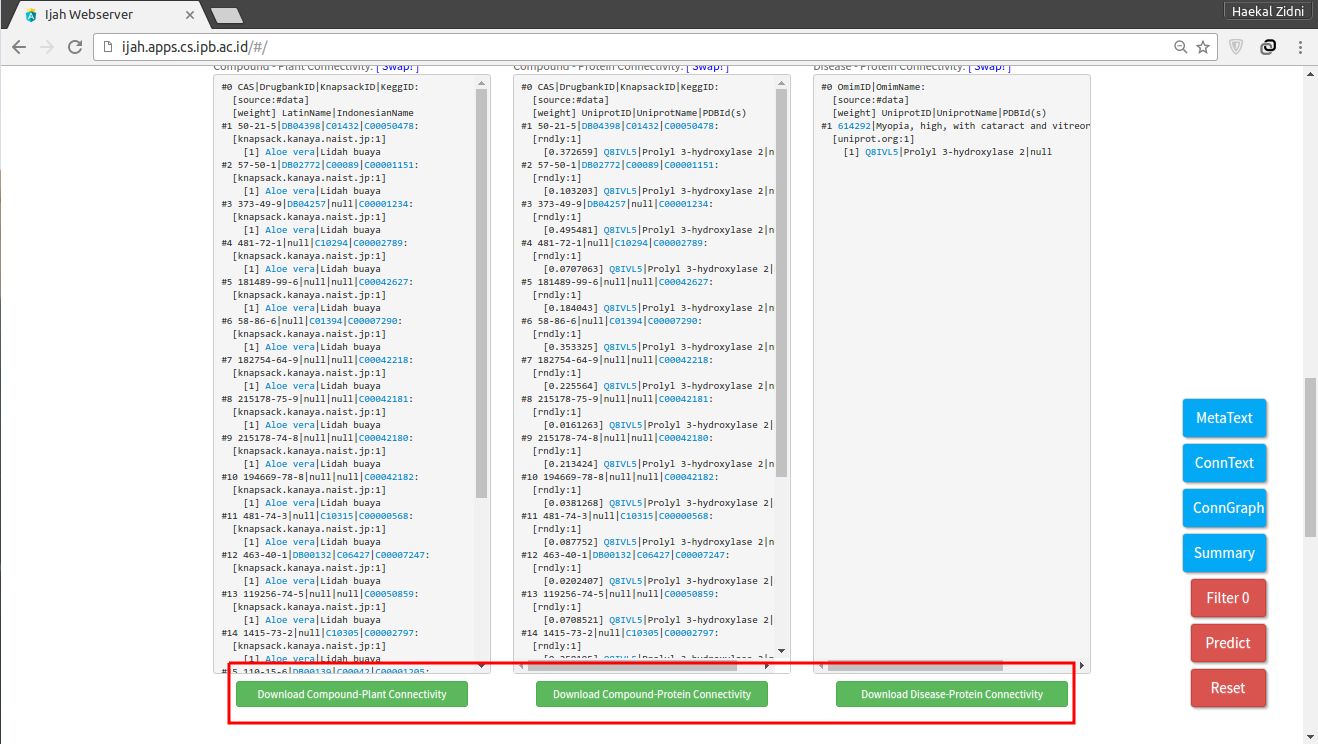
\includegraphics[scale=0.3]{ijah_output_text_download.png}
	\caption{Tombol Download untuk mengunduh file teks konektivitas}
	\label{fig:ijah_output_text_download}
	\end{figure}
	
	\subsection{Metadata Text} \label{meta}
	Metadata Text berisi metadata (nama dan ID) dari semua entitas yang terlibat dalam proses ini. Pada bagian bawah, juga terdapat tombol Download untuk mengunduh teks Metadata ini.

	\begin{figure}[H]
	\centering
	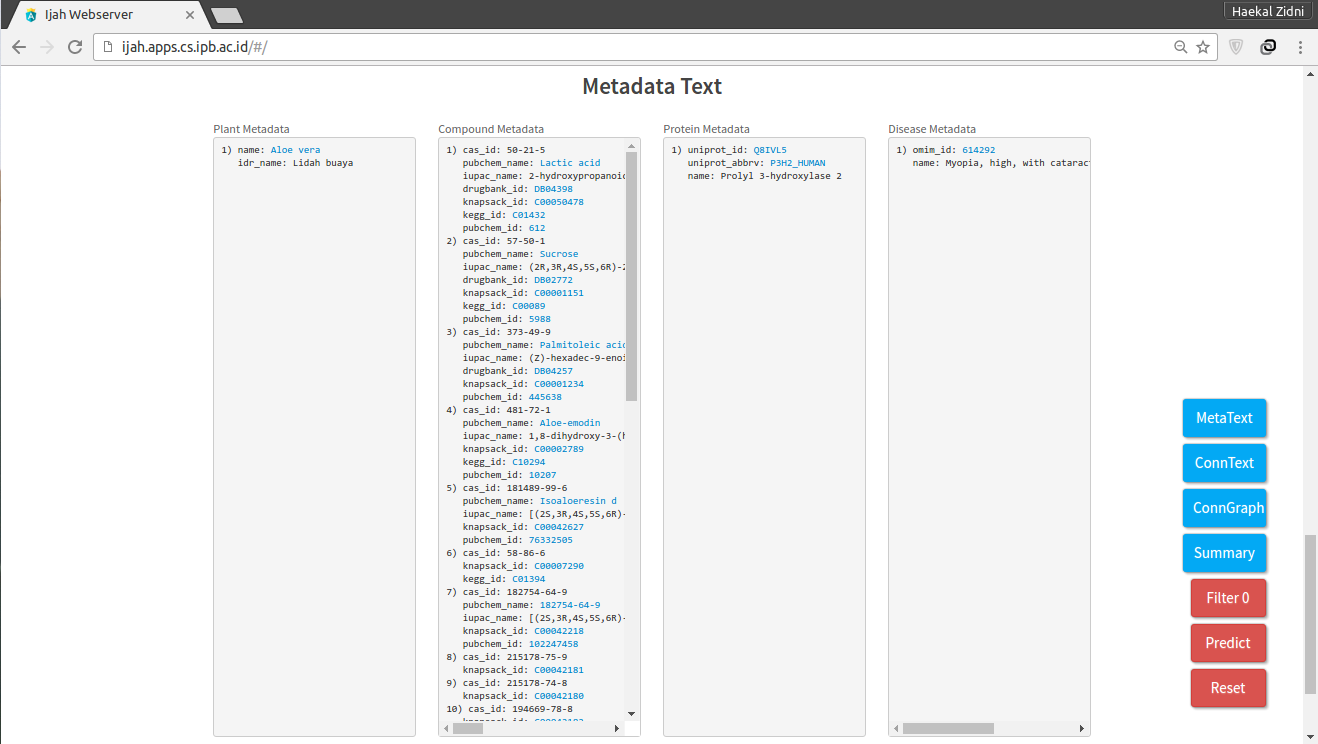
\includegraphics[scale=0.3]{ijah_output_meta.png}
	\caption{Metadata Text Output pada Ijah Webserver}
	\label{fig:ijah_output_meta}
	\end{figure}

	\begin{figure}[H]
	\centering
	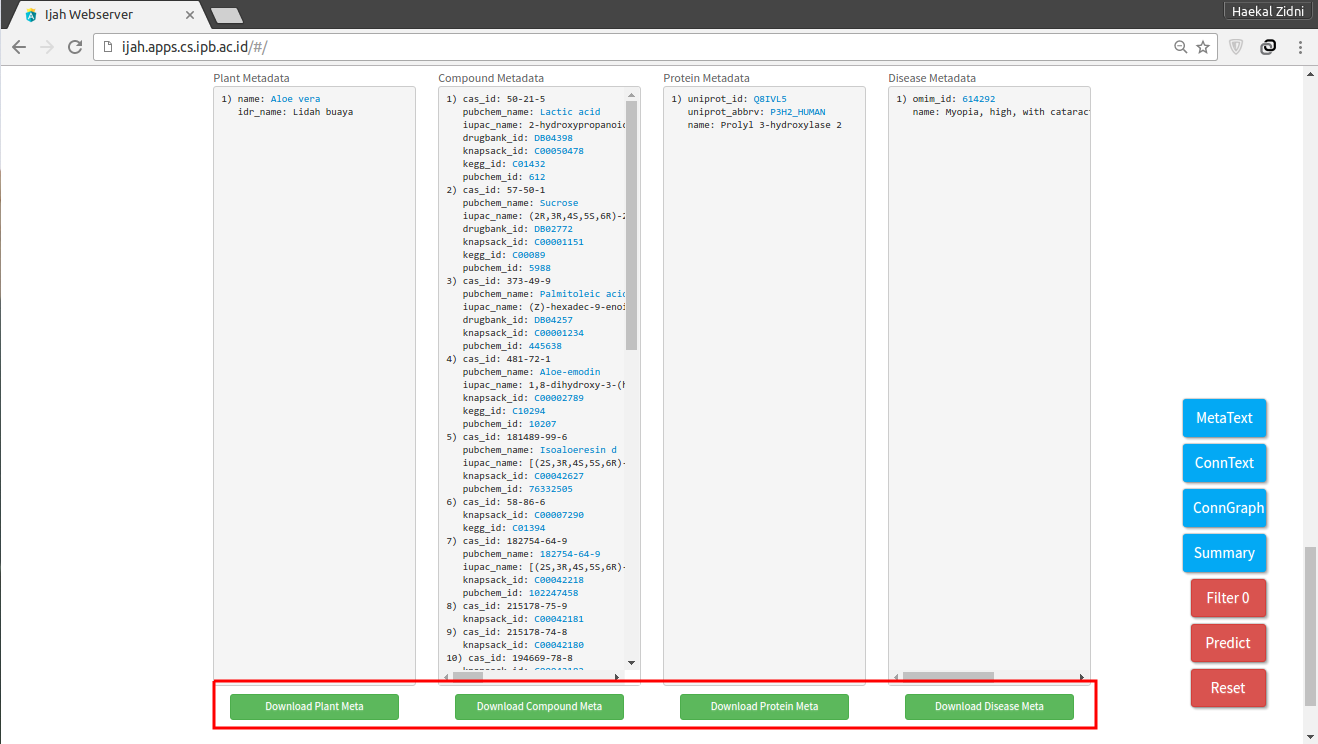
\includegraphics[scale=0.3]{ijah_output_meta_download.png}
	\caption{Tombol Download untuk mengunduh file teks Metadata}
	\label{fig:ijah_output_meta_download}
	\end{figure}


\section{Memodifikasi Output}
Pada halaman output, terdapat \emph{floating button} di sisi kanan bawah yang berisi beberapa fungsi.

	\begin{figure}[H]
	\centering
	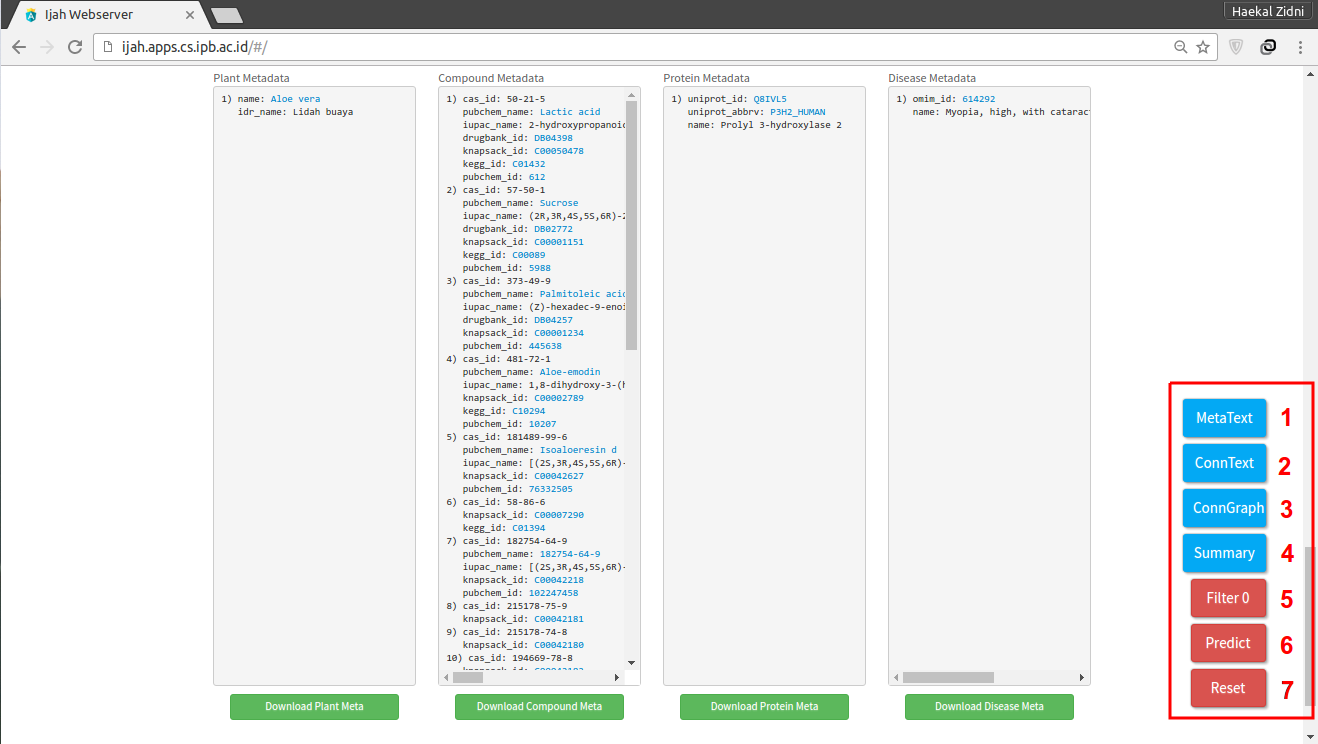
\includegraphics[scale=0.3]{ijah_floating.png}
	\caption{Floating button pada Ijah Webserver}
	\label{fig:ijah_floating}
	\end{figure}

Tombol-tombol pada \emph{floating button} beserta fungsinya:
\begin{enumerate}
\item \textbf{MetaText:} jalan pintas menuju \hyperref[meta]{\textbf{Metadata Text Output}}
\item \textbf{ConnText:} jalan pintas menuju \hyperref[text]{\textbf{Connectivity Text Output}}
\item \textbf{ConnGraph:} jalan pintas menuju \hyperref[graph]{\textbf{Connectivity Graph Output}}
\item \textbf{Summary:} jalan pintas menuju \hyperref[summary]{\textbf{Summary}}
\item \textbf{Filter:} akan dibahas pada bagian \hyperref[filter]{\textbf{Filter}}
\item \textbf{Predict:} akan dibahas pada bagian \hyperref[predictmore]{\textbf{Predict}}
\item \textbf{Reset:} mengosongkan seluruh hasil proses dan mengulang ke halaman awal.
\end{enumerate}

	\subsection{Filter} \label{filter}
	Tombol Filter berfungsi untuk menyaring skor konektivitas yang akan ditampilkan. Filter ini memiliki beberapa level yaitu:
	\begin{itemize}
	\item 0 - Menampilkan keseluruhan konektivitas yang ada (minimum skor 0).
	\item 0.2 - Menampilkan konektivitas dengan skor diatas 0.2
	\item 0.4 - Menampilkan konektivitas dengan skor diatas 0.4
	\item 0.6 - Menampilkan konektivitas dengan skor diatas 0.6
	\item 0.8 - Menampilkan konektivitas dengan skor diatas 0.8
	\item 1 - Menampilkan konektivitas yang benar2 terhubung 100\% \emph{known by experiment} (skor 1).
	\end{itemize}

	\begin{figure}[H]
	\centering
	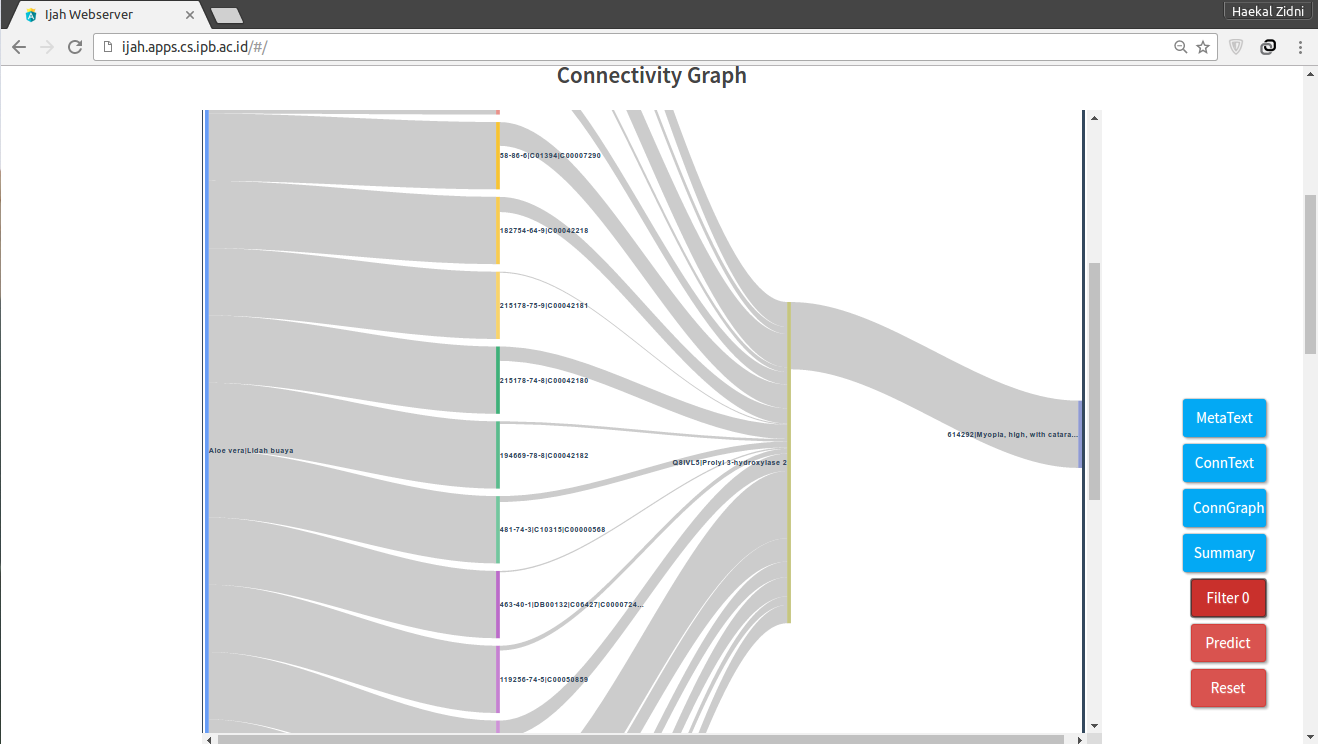
\includegraphics[scale=0.3]{ijah_filter_0.png}
	\caption{Filter 0, menampilkan semua konektivitas}
	\label{fig:ijah_filter_0}
	\end{figure}

	\begin{figure}[H]
	\centering
	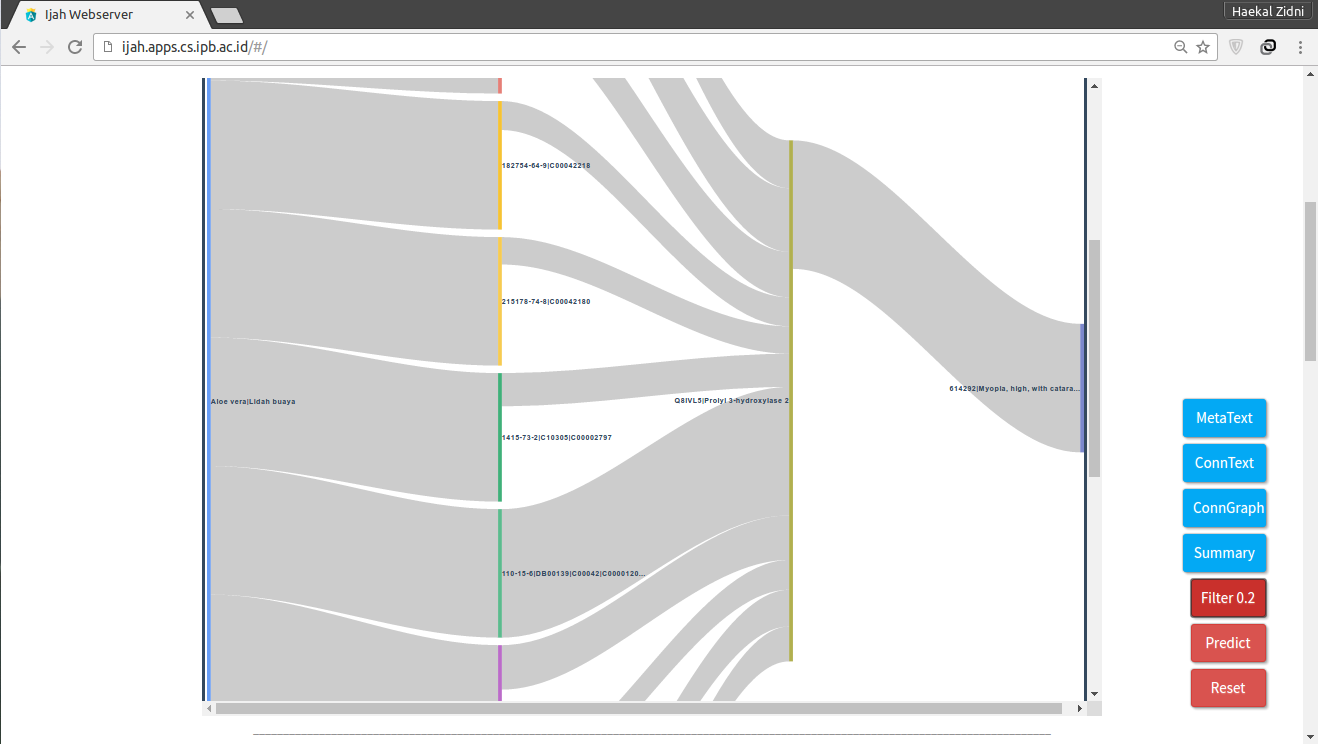
\includegraphics[scale=0.3]{ijah_filter_02.png}
	\caption{Filter 0.2, menampilkan konektivitas diatas 0.2, output mulai berkurang}
	\label{fig:ijah_filter_02}
	\end{figure}

	\begin{figure}[H]
	\centering
	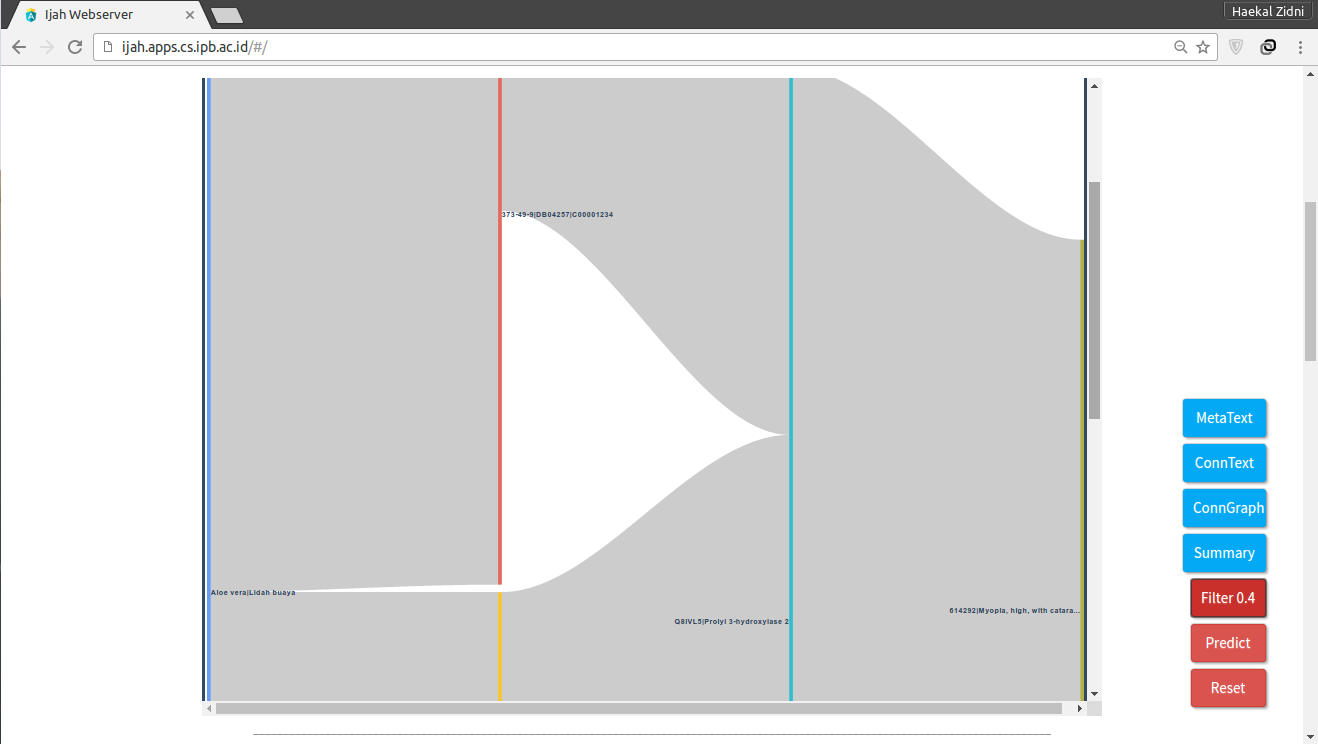
\includegraphics[scale=0.3]{ijah_filter_04.png}
	\caption{Filter 0.4, menampilkan konektivitas diatas 0.4, output jauh berkurang karena konektivitas dengan skor diatas 0.4 semakin sedikit}
	\label{fig:ijah_filter_04}
	\end{figure}

	\begin{figure}[H]
	\centering
	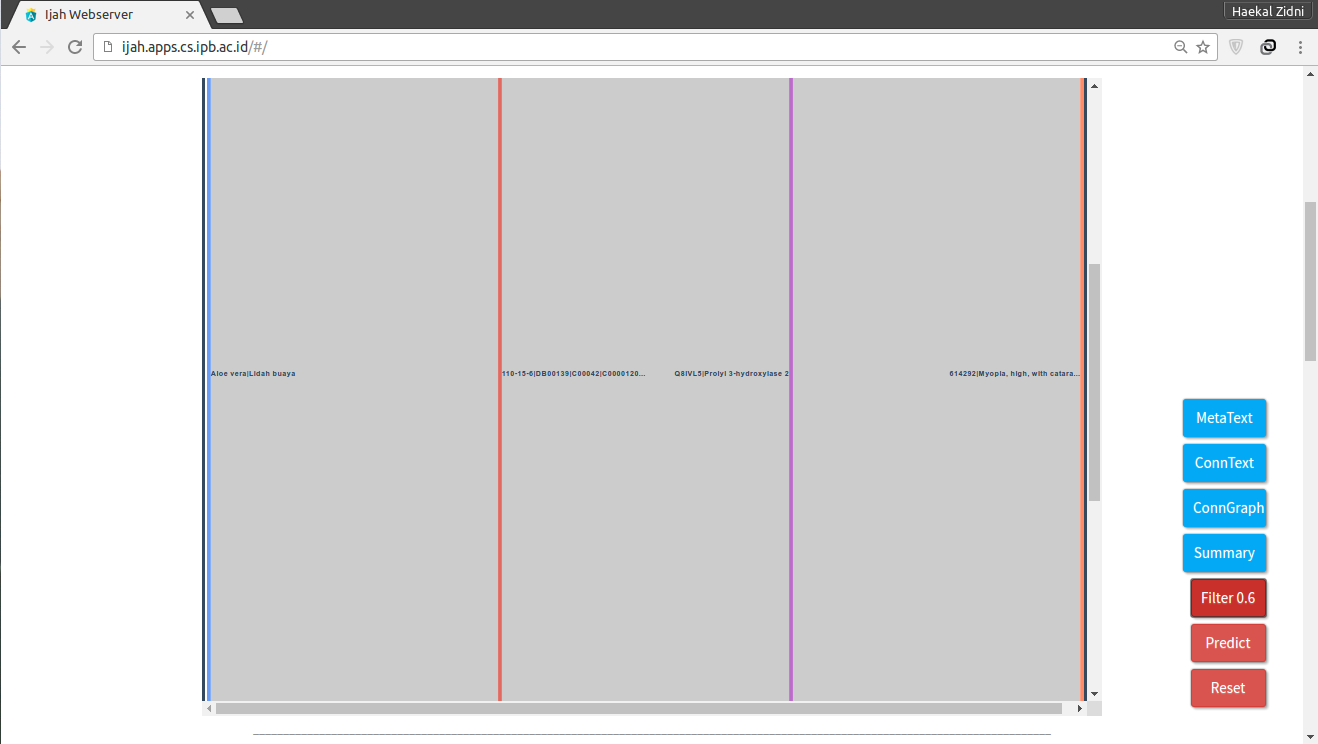
\includegraphics[scale=0.3]{ijah_filter_06.png}
	\caption{Filter 0.6, menampilkan konektivitas diatas 0.6, hanya ada satu output yang muncul. Dalam kasus ini output yang tersisa hanya yang bernilai 1 (100\% terkoneksi) sehingga filter 0.8 dan filter 1 memunculkan hasil yang sama}
	\label{fig:ijah_filter_02}
	\end{figure}

	\subsection{Predict} \label{predictmore}
	Ketika tombol eksekusi dijalankan, ada batas waktu prediksi 5 detik. Terkadang belum semua prediksi termuat pada saat output muncul, sehingga tombol \textbf{Predict} memberikan kesempatan untuk melanjutkan prediksi kembali selama 5 detik. Output yang dihasilkan mungkin akan bertambah seiring bertambahnya hasil prediksi.

	\begin{figure}[H]
	\centering
	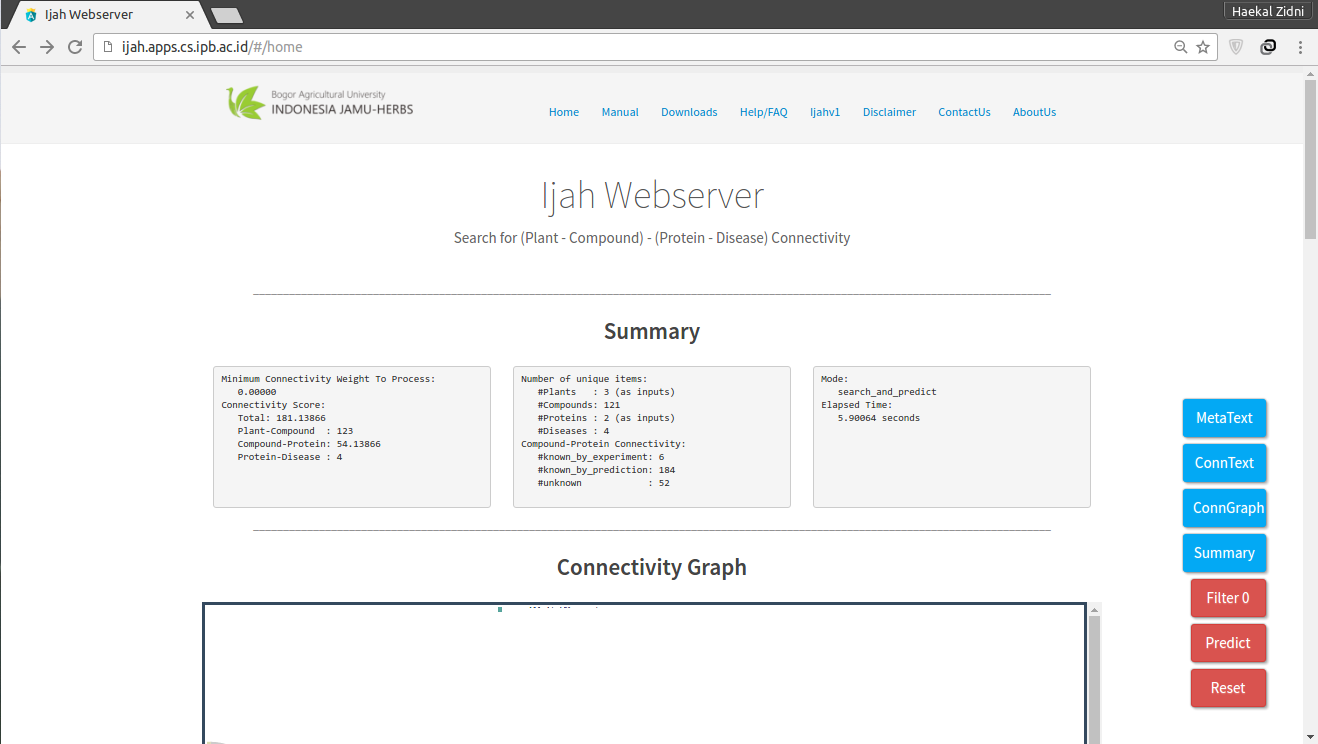
\includegraphics[scale=0.3]{ijah_predict_01.png}
	\caption{Salah satu contoh output. Nilai awal yaitu Known By Prediction sebanyak 184, dengan nilai konektivitas yang belum diketahui (Unknown) sebesar 52}
	\label{fig:ijah_predict_01}
	\end{figure}

	\begin{figure}[H]
	\centering
	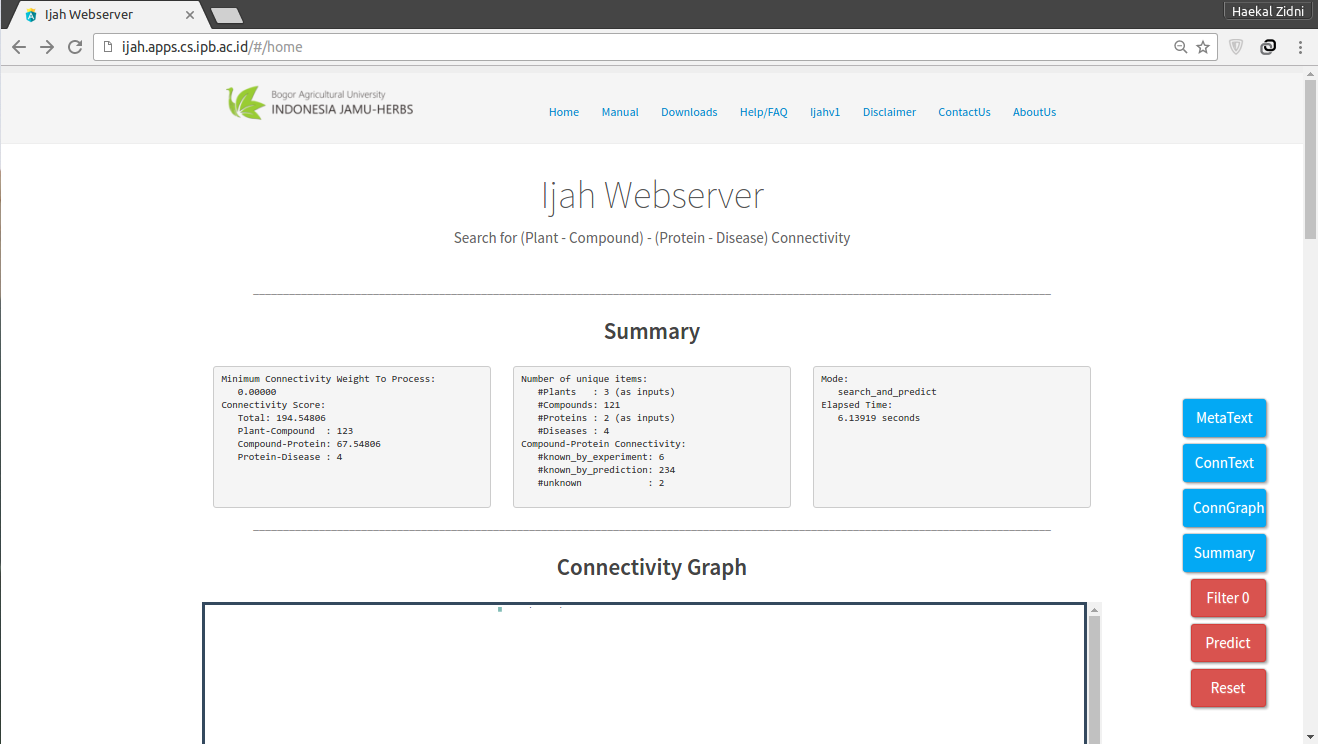
\includegraphics[scale=0.3]{ijah_predict_02.png}
	\caption{Setelah dijalankan tombol Predict dan melakukan 5 detik prediksi tambahan, nilai Known By Prediction meningkat menjadi 234 dan Unknown berkurang hingga tersisa 2 saja}
	\label{fig:ijah_predict_02}
	\end{figure}
